% iaus2esa.tex -- sample pages for Proceedings IAU Symposium document class
% (based on v1.0 cca2esam.tex)
% v1.04 released 17 May 2004 by TechBooks
%% small changes and additions made by KAvdH/IAU 4 June 2004
% Copyright (2004) International Astronomical Union

\NeedsTeXFormat{LaTeX2e}

\documentclass{iaus}
\usepackage{graphicx}

\title[JD 11.~~Pre-solar grains and AGB stars] %% give here short title %%
{What can pre-solar grains tell us \\ about AGB stars?}

\author[Maria A. Lugaro \& Susanne H{\"o}fner]   %% give here short author list %%
{Maria A. Lugaro$^1$
%%  \thanks{Present address: Fluid Mech Inc., 24 The Street, Lagos, Nigeria.},
 \and Susanne H{\"o}fner$^2$}

\affiliation{$^1$Sterrenkundig Instituut, University of Utrecht, \\ Postbus 80000,
NL-3508TA, Utrecht, the Netherlands \\ email: {\tt m.lugaro@phys.uu.nl} \\[\affilskip]
$^2$Dept. of Astronomy \& Space Physics, Uppsala University, \\ Box
515, SE-75120 Uppsala, Sweden \\email: {\tt hoefner@astro.uu.se}}

\pubyear{2008}
\volume{xxx}  %% insert here IAU Symposium No.
\pagerange{119--126}
% \date{?? and in revised form ??}
\setcounter{page}{119}
\jname{Title of your IAU Symposium}
\editors{A.C. Editor, B.D. Editor \& C.E. Editor, eds.}
\begin{document}

\maketitle

\begin{abstract}
Small amounts of pre-solar grains have survived in the matrices of primitive meteorites
and interplanetary dust particles. Their detailed study in the laboratory with modern
analytical tools provides highly accurate and detailed information with regard to stellar
nucleosynthesis and evolution, grain formation in stellar atmospheres, and Galactic
Chemical Evolution. Their survival puts constraints on conditions they were exposed
to in the interstellar medium and in the Early Solar System.
\keywords{Keyword1, keyword2, keyword3, etc.}
%% add here a maximum of 10 keywords, to be taken form the file <Keywords.txt>
\end{abstract}

\firstsection % if your document starts with a section,
              % remove some space above using this command.
\section{Introduction}

Almost twenty years have passed since, as a result of the search for host phases of
isotopically unusual noble gases, the first discovery in 1987 of surviving pre-solar minerals
(diamond and silicon carbide) in primitive meteorites. These were followed by others
(graphite, refractory oxides, silicon nitride, and finally silicates) in the years since. Pre-solar
grains occur in even higher abundance than in meteorites in interplanetary dust particles
(IDPs). The result is a kind of `new astronomy' based on the study of pre-solar condensates
with all the methods available in modern analytical laboratories.

In the `classical' approach, pioneered in the search for the noble gas carriers diamond,
SiC and graphite, pre-solar grains are isolated by dissolving most of the meteorites (consisting
mostly of silicate minerals) using strong acids, followed by further chemical and physical
separation methods. For overviews at the early stage when only these types were known see
reviews by 
\cite[Anders \& Zinner (1993)]{AndersZinner93} and 
\cite[Ott (1993)]{Ott93}.

More up-to-date reviews (although only barely including the only recently found pre-
solar silicates) are by 
\cite[Zinner (1998)]{Zinner98}, 
\cite[Hoppe \& Zinner (2000)]{HoppeZinner00}, 
\cite[Nittler (2003)]{Nittler03}, and 
\cite[Zinner (2004)]{Zinner04}. 
Refractory oxides and silicon nitride were found in conjunction with the noble gas
carrying minerals because of their similar chemical inertness which allowed them to survive
the extraction procedure of the noble gas carriers. Identification of pre-solar silicates among
the sea of `normal silicates', however, became possible only with the advent of a new
generation of analytical instrumentation, the NanoSIMS (e.g., 
\cite[Hoppe et al. 2004]{Hoppe_etal04}) that allowed
the imaging search for isotopically anomalous phases in situ, i.e. without the need for
chemical / physical extraction.

Central to the identification of pre-solar minerals is the determination of isotopic
compositions, which as a rule strongly deviate from the normal (Solar System) composition.
Isotopic composition is, as a matter of fact, the main (and only safe) criterion by which they
can be identified; hence all our known `pre-solar grains' are `circum-stellar condensates' that
carry the isotopic signatures of nucleosynthesis processes going on in their parent stars
(Fig.\,\ref{fig1}).

Because pre-solar grains come from different stellar sources, information on individual
stars can only be obtained by the study of single grains. This is possible by SIMS (Secondary
Ion Mass Spectrometry) for the light to intermediate-mass elements, RIMS (Resonance
Ionization Mass Spectrometry) for the heavy elements, and laser heating and gas mass
spectrometry for He and Ne.

\begin{figure}[b]
% \vspace*{-2.0 cm}
\begin{center}
 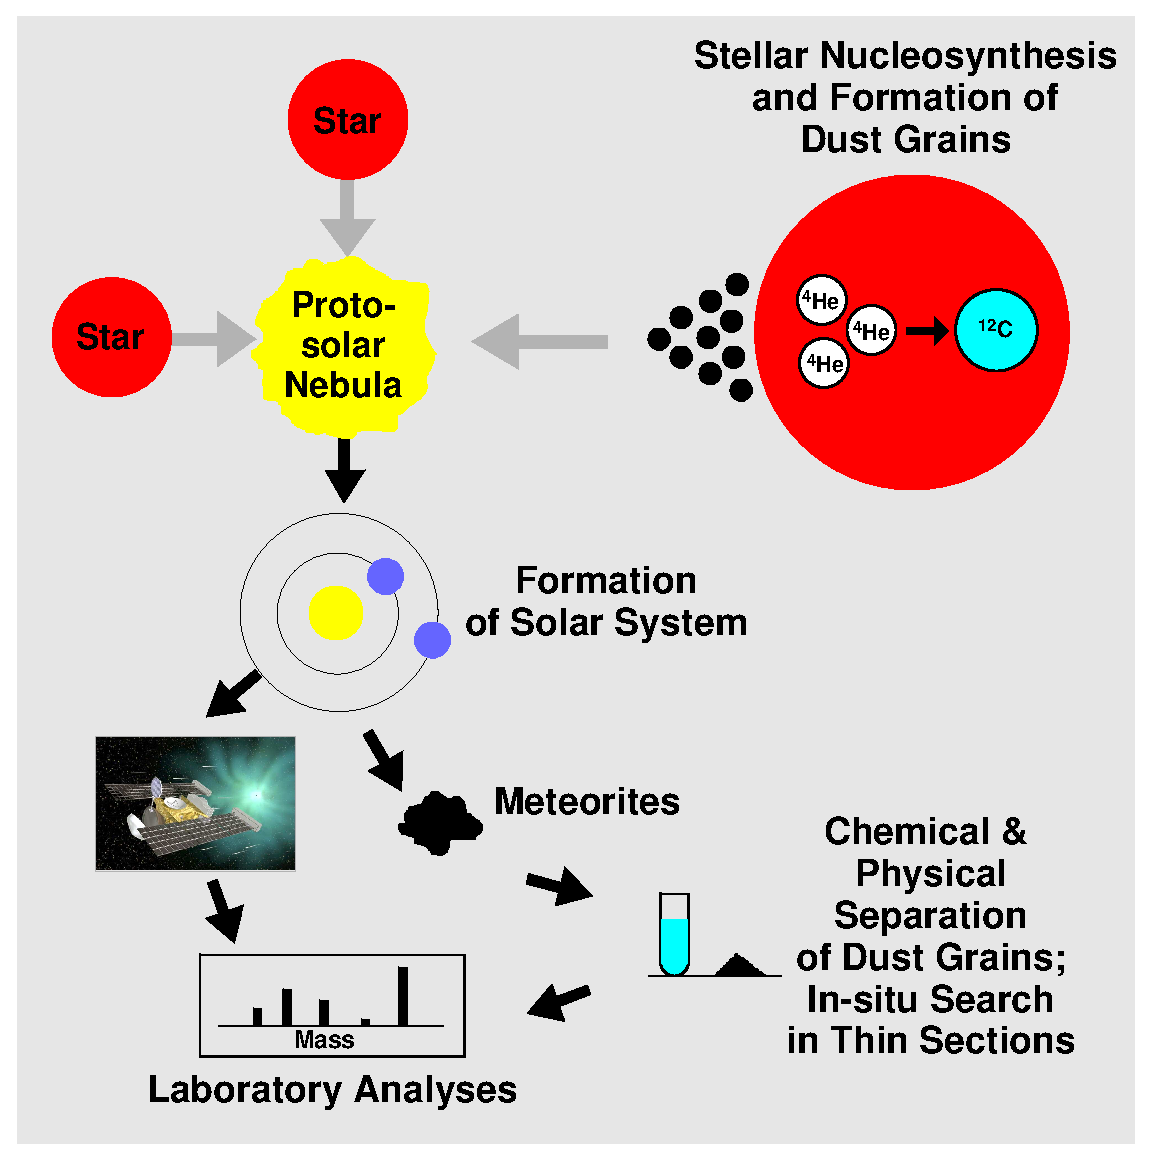
\includegraphics[width=3.4in]{Path.eps} 
% \vspace*{-1.0 cm}
 \caption{Path of pre-solar grains from their stellar sources to the laboratory.}
   \label{fig1}
\end{center}
\end{figure}

\section{Overview}

An overview of the currently known inventory of circumstellar grains in meteorites is
presented in Table \ref{tab1}. Abundances of silicates are definitely, those of the other pre-solar
grains most likely, higher in IDPs. Some comments follow below, while several specific cases
are discussed in detail in other contributions to this volume.

 
\begin{table}
  \begin{center}
  \caption{Overview of current knowledge on circum-stellar condensate grains in meteorites.}
  \label{tab1}
 {\scriptsize
  \begin{tabular}{|l|c|c|c|c|}\hline 
{\bf Mineral} & {\bf Size [$\mu$m]} & {\bf Isotopic Signatures} & {\bf Stellar} & {\bf Contri-} \\ 
   &  {\bf abund.}  [ppm]$^1$ & & {\bf Sources} & {\bf bution$^2$} \\ \hline
diamond & $~0.0026$ & Kr-H, Xe-HL, Te-H & supernovae & ? \\
   & ~1500 & & & \\ \hline
silicon & $~0.1-10$ & enhanced $^{13}$C, $^{14}$N, $^{22}$Ne, s-process elem. & AGB stars & $> 90$~\% \\
carbide & $~30$ & low $^{12}$C/$^{13}$C, often enh.\ $^{15}$N & J-type C-stars (?) & $< 5$~\% \\
 & & enhanced $^{12}$C, $^{15}$N, $^{28}$Si; extinct $^{26}$Al, $^{44}$Ti & Supernovae & 1~\% \\
 & & low $^{12}$C/$^{13}$C, low $^{14}$N/$^{15}$N & novae &  $0.1$~\% \\ \hline
graphite & $~0.1-10$ & enh.\ $^{12}$C, $^{15}$N, $^{28}$Si; extinct $^{26}$Al, $^{41}$Ca, $^{44}$Ti &
 SN (WR?) & $< 80$~\% \\ 
 & $~10$ & s-process elements & AGB stars & $> 10$~\% \\
 & & low $^{12}$C/$^{13}$C  & J-type C-stars (?) & $< 10$~\% \\
 & & low $^{12}$C/$^{13}$C; Ne-E(L) & novae & 2~\% \\ \hline
 corundum/ & $~0.1-5$ & enhanced $^{17}$O, moderately depl. $^{18}$O & RGB / AGB & $> 70$~\% \\
 spinel/ & $~50$ & enhanced $^{17}$O, strongly depl. $^{18}$O & AGB stars & 20~\% \\
 hibonite & & enhanced $^{16}$O & supernovae & 1~\% \\ \hline
 silicates & $~0.1-1$ & similar to oxides above & & \\
 &  $~140$ & & & \\ \hline
 silicon & $~1$ & enhanced $^{12}$C, $^{15}$N, $^{28}$Si; extinct $^{26}$Al & supernovae & 100~\% \\
 nitride & $~ 0.002$ & & & \\ \hline
  \end{tabular}
  }
 \end{center}
\vspace{1mm}
 \scriptsize{
 {\it Notes:}\\
  $^1$For the abund.\ (in wt.\ ppm) the reported maximum values from different meteorites are given. \\
  $^2$Note uncertainty about actual fraction of diamonds that are pre-solar and for fraction of graphite attributed to SN and AGB stars (see discussion in text).}
\end{table}

{\underline{\it Silicon carbide}}. All SiC grains in primitive meteorites are of pre-solar origin, and they are
the best characterized. This has been helped by their comparably high contents of minor and
trace elements. Characteristic for most grains are enhanced $^{13}$C, $^{14}$N, former presence of $^{26}$Al
as indicated by overabundances of its daughter $^{26}$Mg, neon that is almost pure $^{22}$Ne 
[Ne-E(H)]
and heavy elements showing the characteristic isotopic signatures of the s-process. These
`mainstream grains' quite obviously are condensates out of the winds of AGB stars (see
contribution by Lugaro \& H{\"o}fner, this volume). Only a percent or so have a clearly different origin tied to
supernovae (the `X-grains'). They are characterized by high $^{12}$C, $^{28}$Si, very high former
abundances of $^{26}$Al as well as $^{44}$Ti and not fully understood signature in the heavy trace
elements (see contribution by Amari \& Lodders, this volume).

{\underline{\it Oxides and silicates}}. Besides diamonds (see below) silicates - not unexpectedly - are the
most abundant of the pre-solar grains that have been found. The most characteristic features
of oxides and silicates are contained in the oxygen isotopic composition that can be used for
assigning each grain to one of four groups 
(\cite[Nittler et al. 1997]{Nittler_etal97}). Grains without evidence for
the former presence of $^{26}$Al are assumed to originate from RGB stars, those with $^{26}$Al from AGB stars.

{\underline{\it Graphite and silicon nitride}}. The characteristics of most grains (see Tab.\,\ref{tab1}) have
traditionally led to assume a SN origin (e.g., 
\cite[Zinner 1998]{Zinner98}; 
\cite[Hoppe \& Zinner 2000]{HoppeZinner00}). 
However,
this percentage may have been overestimated as most high-density graphite grains, although
showing enhanced $^{12}$C abundances, contain s-process signatures and so are more likely to
originate from AGB stars 
(\cite[Croat et al.  2005]{Croat_etal05}). The rare Si$_3$N$_4$ grains show isotopic signatures
similar to SiC-X and SN graphite grains and derive probably from supernovae as well.

{\underline{\it Nanodiamonds}}. In several ways these are the most enigmatic. Although discovered first,
their pre-solar credentials are based solely on trace elements Te and noble gases that they
carry. They are too small for individual analysis � each consisting of some 1000 carbon atoms
only on average and the carbon isotopic composition of `bulk samples' (i.e., many diamond
grains) is within the range of Solar System materials. What fraction of the diamonds is truly
pre-solar is an as yet open question.

\section{Implications}

{\underline{\it Isotopic structures and nucleosynthesis}}. As isotopic structures are the key for
establishing the grains as pre-solar, isotope studies are at the core of investigations that have
been performed. Results from isotopic studies in turn are also those that bear strongest on
astrophysics. For one, they allow us to pinpoint the grains' stellar sources. In addition, given the
precision of the laboratory isotopic analyses, which far exceed whatever can be hoped for in
remote analyses, they allow conclusions with regard to details of nucleosynthesis and mixing
in the parent stars as well as Galactic Chemical Evolution. They have borne strong on, e.g. the
need for an extra mixing process (cool bottom processing) in Red Giants and provide detailed
constraints on the operation of the s-process in AGB stars (e.g., 
\cite[Busso et al. 1999]{Busso_etal99}). 
A non-standard neutron capture process (`neutron burst') may be implied by the SiC-X grains from supernovae 
(\cite[Meyer et al. 2000]{Meyer_etal00}) and possibly the trace Xe in the diamonds (e.g., 
\cite[Ott 2002]{Ott02}).
The progress in analytical techniques promises more important results in the near future.

{\underline{\it Grain formation}}. Chemical composition, sizes, and microstructures of grains constrain
conditions during condensation in stellar winds and supernova ejecta. Condensation of SiC
apparently occurred under close to the equilibrium conditions (e.g., 
\cite[Lodders \& Fegley 1998]{LoddersFegley98}).
Additional constraints are imposed by trace element contents both on average 
(\cite[Yin et al. 2006]{Yin_etal06}) 
as well as in individual grains 
(\cite[Amari et al. 1995]{Amari_etal95}). 
An important relevant observation is
the occurrence of subgrains of primarily TiC within graphite 
(\cite[Croat et al. 2005]{Croat_etal05}).

{\underline{\it The lifecycle of pre-solar grains (and maybe interstellar grains in general)}}. Interstellar grains
are expected to be processed and eventually destroyed by sputtering or astration (e.g.,
\cite[Draine 2003]{Draine03}), with an as yet unidentified process needed to account for the balance between
formation and destruction. Pre-solar grains preserved in meteorites carry, in principle, a
record of conditions they have been exposed to, which, however, is difficult to read.
Determining an absolute age using long-lived radioisotopes is virtually ruled out by the fact
that these systems use decay of rare constituents (e.g., K, Sr, Re, U) decaying into other rare
elements with uncertain non-radiogenic composition. However, appearance and
microstructures of pristine (i.e. not chemically processed) SiC show little evidence for being
processed, indicating either that they were surprisingly young when entering the forming
Solar System or that they were protected 
(\cite[Bernatowicz et al. 2003]{Bernatowicz_etal03}); a similar situation is
indicated by the lack of detectable spallation Xe produced by exposure to cosmic rays during residence in the ISM 
(\cite[Ott et al.  2005]{Ott_etal05}). The distribution, finally, among various types of
meteorites, provides a measure of processing in the early Solar System.

\begin{thebibliography}{}

\bibitem[Amari \etal\ (1995)]{Amari_etal95}
{Amari, S., Hoppe, P., Zinner, E., \& Lewis R.S.} 1995,
\textit{Meteoritics}, 30, 490 

\bibitem[Anders \& Zinner (1993)]{AndersZinner93}
{Anders, E., \& Zinner, E.} 1993, 
\textit{Meteoritics}, 28, 490

\bibitem[Bernatowicz et al. (2003)]{Bernatowicz_etal03}
{Bernatowicz, T.J., Messenger, S., Pravdivtseva, O., Swan, P., \& Walker, R.M.} 2003, 
\textit{Geochim. Cosmochim. Acta}, 67, 4679

\bibitem[Busso et al. (1999)]{Busso_etal99}
{Busso, M., Gallino, R., \& Wasserburg, G.J.} 1999, 
\textit{ARAA}, 37, 239

\bibitem[Croat, Stadermann \& Bernatowicz (2005)]{Croat_etal05}
{Croat, T.K., Stadermann, F.J., \& Bernatowicz, T.J.} 2005, 
\textit{ApJ}, 631, 976

\bibitem[Draine (2003)]{Draine03}
{Draine, B.T.} 2003,
\textit{ARAA}, 41, 241

\bibitem[Hoppe \& Zinner (2000)]{HoppeZinner00}
{Hoppe, P., \& Zinner, E.} 2000, 
\textit{J. Geophys. Res.}, A105, 10371

\bibitem[Hoppe, Ott \& Lugmair (2004)]{Hoppe_etal04}
{Hoppe, P., Ott, U., \& Lugmair, G.W.} 2004, 
\textit{New Astron. Revs}, 48, 171

\bibitem[Lodders \& Fegley (1998)]{LoddersFegley98}
{Lodders, K., \& Fegley, B.} 1998, 
\textit{Meteorit. Planet. Sci.}, 33, 871

\bibitem[Meyer, Clayton \& The (2000)]{Meyer_etal00}
{Meyer, B.S., Clayton, D.D., \& The, L.-S.} 2000, 
\textit{ApJ} (Letters), 540, L49

\bibitem[Nittler (2003)]{Nittler03}
{Nittler, L.R.} 2003, 
\textit{Earth Planet. Sci. Lett.}, 209, 259

\bibitem[Nittler et al. (1997)]{Nittler_etal97}
{Nittler, L.R., Alexander, C.M.O'D., Gao, X., Walker, R.M., \& Zinner, E.} 1997,
\textit{ApJ}, 483, 475

\bibitem[Ott (1993)]{Ott93}
{Ott, U.} 1993, 
\textit{Nature}, 364, 25

\bibitem[Ott (2002)]{Ott02}
{Ott, U.} 2002,
\textit{New Astron. Revs} 46, 513

\bibitem[Ott et al. (2005)]{Ott_etal05}
{Ott, U., Altmaier, M., Herpers, U., Kuhnhenn, J., Merchel, S., 
Michel, R., \& Mohapatra, R.K.} 2005, 
\textit{Meteorit. Planet. Sci.}, 40, 1635

\bibitem[Yin, Lee \& Ott (2006)]{Yin_etal06}
{Yin, Q.-Z., Lee, C.-T. A., \& Ott, U.} 2006, 
 \textit{ApJ}, 647, 676

\bibitem[Zinner (1998)]{Zinner98}
{Zinner, E.} 1998,
 \textit{Ann. Rev. Earth Planet. Sci.}, 26, 147

\bibitem[Zinner (2004)]{Zinner04}
{Zinner, E.} 2004, in: K.K. Turekian, H.D. Holland \& A.M. Davis (eds.), 
 \textit{Treatise in Geochemistry 1} (Oxford and San Diego: Elsevier), p.\,17

\end{thebibliography}

\begin{discussion}

\discuss{Massey}{I�m wondering if you have considered the expected intrinsic dispersion in absolute
magnitude of WRs --� if you consider the (large) mass range that becomes an
early WN or late WC according to the evolutionary models, wouldn�t you expect a large
dispersion in M$_v$?}

\discuss{van der Hucht}{Indeed, we will be always left with some intrinsic scatter in M$_v$ due
to mass differences within the same spectral subtype. But in my opinion, the current
large dispersion is for a large fraction due to incertainties of the adopted distances of
open clusters and OB associations.}

\discuss{Walborn}{I think that the scatter in WNL absolute magnitudes is dominated by intrinsic
spread rather than errors. In the LMC, one finds a range of $�5$ to nearly $�8$. This
in turn likely reflects different formation channels: mass-transfer binaries, post-RSG,
and extremely massive stars in giant H {\scshape ii} regions.}

\discuss{van der Hucht}{As said above, there is likely to be intrinsic scatter. But, I wonder
whether a scatter of 3 magnitudes perhaps reflects undetected
multiplicity.} 

\discuss{Ma\'{\i}z-Apell\'{a}niz}{I could not agree more with your comment on the need for an updated
catalogue of O-type stars (as a follow up of that of Garmany
{\itshape et al.} 1982). We
are currently working on precisely that (see our poster, these Proceedings) and we will
soon make it available.}

\discuss{van der Hucht}{Wonderful.}

\discuss{Koenigsberger}{Is the ratio WR/O-stars in clusters similar or different from this ratio
for the field stars?}

\discuss{van der Hucht}{I think it is different because incompleteness among field stars is even
larger than that among cluster stars. But perhaps it should also be different because
WR stars are older and could have drifted away from clusters, more
than O-type stars.} 

\discuss{Gies}{How many of the WR stars in your catalogue might be low mass objects?}

\discuss{Walborn}{Comment: PN central stars in the WR sample would be only [WC].}

\discuss{van der Hucht}{Among the WR stars in our VIIth Catalogue we doubt only one:
WR109 (V617 Sgr), which is a peculiar object (not even a [WR] central star of a PN).
All other stars in our cataloge are true massive Population I WR stars, and properly
classified as such. We have not listed known Population II [WC] objects, as we did
separately in our VIth Catalogue (van der Hucht {\itshape et al.} 1981). [WN] objects are not
known to exist, see the comment by Nolan.}

\discuss{Zinnecker}{Are all Galactic WR stars in open clusters and OB association or are there
many WR stars in the field?}

\discuss{van der Hucht}{See the VIIth WR catalogue (van der Hucht 2001): of the listed 227
Galactic WR stars, only 53 are in open culsters and OB associations, or believed to be.
The other 184 are supposedly field stars.}
\end{discussion}

\end{document}
